\documentclass[12pt]{article}
\usepackage[T1]{fontenc}
\usepackage[light,math]{iwona}
\usepackage[latin1]{inputenc}
\usepackage{amsmath}
\usepackage{mathtools}
\usepackage{xspace}
\usepackage{graphicx}
\usepackage[english]{babel}
\usepackage[font=small,labelfont=bf]{caption}
\usepackage[centering,includeheadfoot,margin=2cm]{geometry}
\usepackage{tikz}
\usetikzlibrary{calc,shapes,arrows,automata,trees,shadows,decorations.pathmorphing,positioning,shapes.misc,shapes.arrows,chains,matrix,scopes,decorations.pathmorphing}
\begin{document}
\title{CS375 WK7}
\author{Jason N Mansfield}
\maketitle
%tikz terminal
\tikzset{
  nonterminal/.style={
    % The shape:
    rounded rectangle,
    % The size:
    minimum size=6mm,
    % The border:
    very thick,
    draw=purple!70!black!50,         % 50% red and 50% black,
                                  % and that mixed with 50% white
    % The filling:
    top color=white,              % a shading that is white at the top...
    bottom color=purple!70!black!20, % and something else at the bottom
    % Font
    font=\itshape
  },
  terminal/.style={
    % The shape:
    diamond,
    minimum size=6mm,
    % The rest
    very thick,draw=black!50,
    top color=white,bottom color=orange!20,
    font=\ttfamily},
  skip loop/.style={to path={-- ++(0,#1) -| (\tikztotarget)}}
}

{
  \tikzset{terminal/.append style={text height=1.5ex,text depth=.25ex}}
  \tikzset{nonterminal/.append style={text height=1.5ex,text depth=.25ex}}
}
%end of tikz terminal stuff

\begin{figure}
\begin{center}
\caption{Q01: FA}
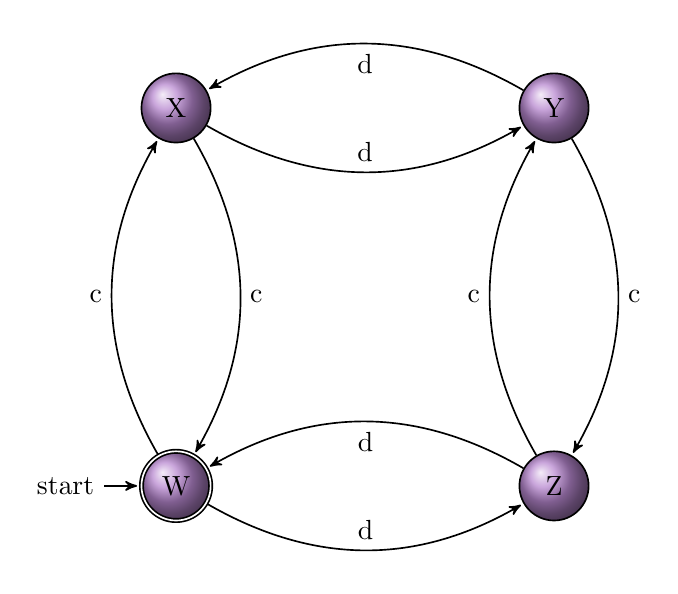
\begin{tikzpicture}[->,>=stealth',shorten >=1pt,auto,node distance=4.8cm, semithick]
\tikzstyle{every state}=[draw=black,text=black, ball color=red!40!blue!47!]
\node[state] (X) {X};
\node[state][right of=X](Y){Y};
\node[state,initial,accepting][below of=X](W){W};
\node[state][below of=Y](Z){Z};
\path (X)edge [bend right] node{d}(Y)
              edge [bend left] node{c}(W)
          (Y)edge [bend right]node{d}(X)
              edge [bend left]node{c}(Z)
          (W)edge [bend left]node{c}(X)
               edge[bend right]node{d}(Z)
          (Z)edge[bend left]node{c}(Y)
              edge[bend right]node{d}(W);      
\end{tikzpicture} 
\end{center}
\end{figure}


\begin{figure}
\begin{center}
\begin{tikzpicture}[node distance=2.8cm,
        point/.style={coordinate},>=stealth',thick,draw=black!50,
        tip/.style={->,shorten >=0.007pt},every join/.style={rounded corners},
        hv path/.style={to path={-| (\tikztotarget)}},
        vh path/.style={to path={|- (\tikztotarget)}},
        text height=1.5ex,text depth=.25ex % align text horizontally
    ]
    %Standard Pushdown Symbols
   \node (start) [nonterminal]   {START};
   \node (accept) [nonterminal]   at (-3,-3.97)  {ACCEPT};
   \node (reject) [nonterminal]   at (9,-6.5) {REJECT};
   \node (reject2) [nonterminal]   at (-3,-6.5) {REJECT};
   %You will need multiple READ and POP Nodes with a varity of names.
   \node (W) [terminal,below=of start]                {READ};
   \node (X) [terminal,right=of W]                      {READ};
   \node (Y) [terminal,below=of X]                     {READ};
   \node (Z) [terminal,below=of W]                     {READ};
   \path (start)   edge[->] (W)  %  simple edges
             (W) edge[->]node[pos=0.50, above]{$\Delta$}(accept)
                   edge[->] node[pos=0.30, above]{c}(X)
                   edge[->] node[pos=0.30, left]{d}(Z);
   \path (X) edge[->] node[pos=0.30,right]{d}(Y);
   \draw [->]
     ( $ (X.north)$)    
     - ++(0,+1.1) 
    node[right]{c}
     -| ($(W.north)$);
  \draw [->]
     ( $ (Z.east)$) -++(1,0) node[right]{d} -++(1,4) -++(-.6,4);
  \draw [->]
     ( $ (Y.east)$) -++(1,0) node[right]{d} -++(1,4) -++(-.6,4);
   \draw [->]
     ( $ (Y.south)$) -++(0,-1) node[below]{c} -| ($(Z.south)$);
  \draw [->]
     ( $ (Z.south)$) -++(4.6,0) node[pos=0.30,above right]{c} ;
  \draw [->]
     ( $ (Z.south)$) -++(-3,0) node[pos=0.70,above right]{$\Delta$} -++(-3,2.7);
  \draw [->]
     ( $ (Y.south)$) -++(4.5,0) node[pos=0.70,above right]{$\Delta$} -++( 4.5,2.7);
 \draw [->]
     ( $ (X.east)$) -++(3.6,0) node[pos=0.70,above right]{$\Delta$} -++( 3.6,-2.2);
      
            

  
\end{tikzpicture}
\end{center}
\end{figure}





\end{document}